\chapter{Results and Analysis}
\label{chap5}

In this chapter we perform synthesis of both cores and run the tests described in \autoref{tab:instr_skip_test} and \autoref{tab:coverage_test} using the steps described in \autoref{subsec:sim_glitch}. The waveforms from simulation of the core are shown for all the tests. In every waveform figure the clock signal is on top, the glitched signal is shown in blue and the alert signals are shown in red on the bottom. Results from the synthesis and tests are discussed in \autoref{sec:discussion}.

\section{PPA comparison}
\label{sec:synth_comparison}

Area and power consumption reports generated after synthesis of both cores are shown in \autoref{tab:cv32e40dc_power} and \autoref{tab:cv32e40s_power}. These tables show the power consumption for several categories. 

\begin{table}[h]
\centering
\caption{Power consumption report for CV32E40DC.}
\label{tab:cv32e40dc_power}
\begin{tabular}{l|cccccc}
\toprule
Category & Leakage [$W$] & Internal [$W$] & Switching [$W$] & Total [$W$] & Row \% \\
\midrule
\rowcolor{black!20} Memory & 0.00 & 0.00 & 0.00 & 0.00 & 0.00\% \\
Register & 3.08383e-06 & 1.62940e-03 & 4.85935e-04 & 2.11842e-03 & 64.79\% \\
\rowcolor{black!20}Latch & 0.00 & 0.00 & 0.00 & 0.00 & 0.00\% \\
Logic & 2.82440e-06 & 3.37798e-04 & 8.10212e-04 & 1.15083e-03 & 35.20\% \\
\rowcolor{black!20}Bbox & 0.00 & 0.00 & 4.76740e-07 & 4.76740e-07 & 0.01\% \\
Clock & 0.00 & 0.00 & 0.00 & 0.00 & 0.00\% \\
\rowcolor{black!20}Pad & 0.00 & 0.00 & 0.00 & 0.00 & 0.00\% \\
Pm & 0.00 & 0.00 & 0.00 & 0.00 & 0.00\% \\
\midrule
\rowcolor{black!20} Subtotal & 5.90822e-06 & 1.96720e-03 & 1.29662e-03 & 3.26973e-03 & 100.00\% \\
Percentage & 0.18\% & 60.16\% & 39.66\% & 100.00\% & 100.00\% \\
\bottomrule
\end{tabular}
\end{table}

\begin{table}[h]
\centering
\caption{Power consumption report for CV32E40S.}
\label{tab:cv32e40s_power}
\begin{tabular}{l|cccccc}
\toprule
Category & Leakage [$W$] & Internal [$W$] & Switching [$W$] & Total [$W$] & Row \% \\
\midrule
\rowcolor{black!20} Memory & 0.00 & 0.00 & 0.00 & 0.00 & 0.00\% \\
Register & 1.24472e-06 & 3.38053e-04 & 1.15429e-04 & 4.54727e-04 & 40.24\% \\
\rowcolor{black!20}Latch & 0.00 & 0.00 & 0.00 & 0.00 & 0.00\% \\
Logic & 1.33087e-06 & 1.70770e-04 & 5.02775e-04 & 6.74876e-04 & 59.72\% \\
\rowcolor{black!20}Bbox & 0.00 & 0.00 & 2.49260e-07 & 2.49260e-07 & 0.02\% \\
Clock & 0.00 & 0.00 & 2.17800e-07 & 2.17800e-07 & 0.02\% \\
\rowcolor{black!20}Pad & 0.00 & 0.00 & 0.00 & 0.00 & 0.00\% \\
Pm & 0.00 & 0.00 & 0.00 & 0.00 & 0.00\% \\
\midrule
\rowcolor{black!20} Subtotal & 2.57559e-06 & 5.08823e-04 & 6.18671e-04 & 1.13007e-03 & 100.00\% \\
Percentage & 0.23\% & 45.03\% & 54.75\% & 100.00\% & 100.00\% \\
\bottomrule
\end{tabular}
\end{table}

\begin{figure}
    \centering
    \includegraphics{powe}
    \caption{Caption}
    \label{fig:enter-label}
\end{figure}

\begin{table}[h]
\centering
\caption{PPA results from simulation and synthesis of both setups.}
\label{tab:ppa_results}
\begin{tabular}{c|ccc}
\toprule 
Setup & Area[$pm^2$] & Power[$\mu W$] & Clock Cycles\\
\midrule
\rowcolor{black!20} CV32E40S & 63121.093 & 113.007 & 18424\\
CV32E40DC & 140587.232[$+122.72\%$] & 326.973[$+189.33\%$] & 18415[$-0.05\%$] \\
\bottomrule
\end{tabular}
\end{table}

From the table we see that the total area and power consumption are increased by $122.72\%$ and $189.33\%$ respectively. From the complete reports we see that the dynamic power consumption from switching increased from $54.75\%$ to $63.42\%$. The amount of clock cycles needed to run the test program decreases by $0.05\%$. This is the same decrease achieved from only removing PCH as shown in \autoref{sec:xsecure}.

The amount of clock cycles each core uses to execute the code from \autoref{lst:test_code} and \autoref{lst:coverage_test} is shown in \autoref{tab:test_ccs}. From the table we see that the CV32E40DC uses 9 fewer clock cycles for each of the tests. This amounts to a decrease of $0.32\%$ and $-0.28\%$ for the instruction skipping test and the fault coverage test repspecively. 

\begin{table}[h]
\centering
\caption{Clock cycle used to execute the code in \autoref{lst:sample_code}, \autoref{lst:test_code} and \autoref{lst:coverage_test} on both cores.}
\label{tab:test_ccs}
\begin{tabular}{c|ccc}
\toprule 
Setup & Sanity test & Instruction skipping & Fault coverage \\
\midrule
\rowcolor{black!20} CV32E40S & 18424 & 2799 & 3132\\
CV32E40DC & 18415[$-0.05\%$] & 2790[$-0.32\%$] & 3123[$-0.28\%$]\\
\bottomrule
\end{tabular}
\end{table}

\section{Instruction Skipping}
\label{sec:instr_skip_result}

\subsection{CV32E40S}
\label{subsec:single_instr_skip}

\subsubsection{Skipping function call}
\label{subsubsec:func_call}

The \textit{c.jal} instruction is logged in the \textit{WB} stage at 1752ns. The fault is injected in the \textit{EX} stage at 1743ns. The program counter is glitched to be \textit{0x0000044e}, thus skipping one instruction. 

Glitching of the core was done successfully, and line \textbf{21} in \autoref{lst:test_code} was executed. The waveforms from simulation are shown in \autoref{fig:instr_skip_single_wave}. From the figure one can see that the glitch is detected immediately and a major alert is raised. 

\begin{figure}[h!]
    \centering
    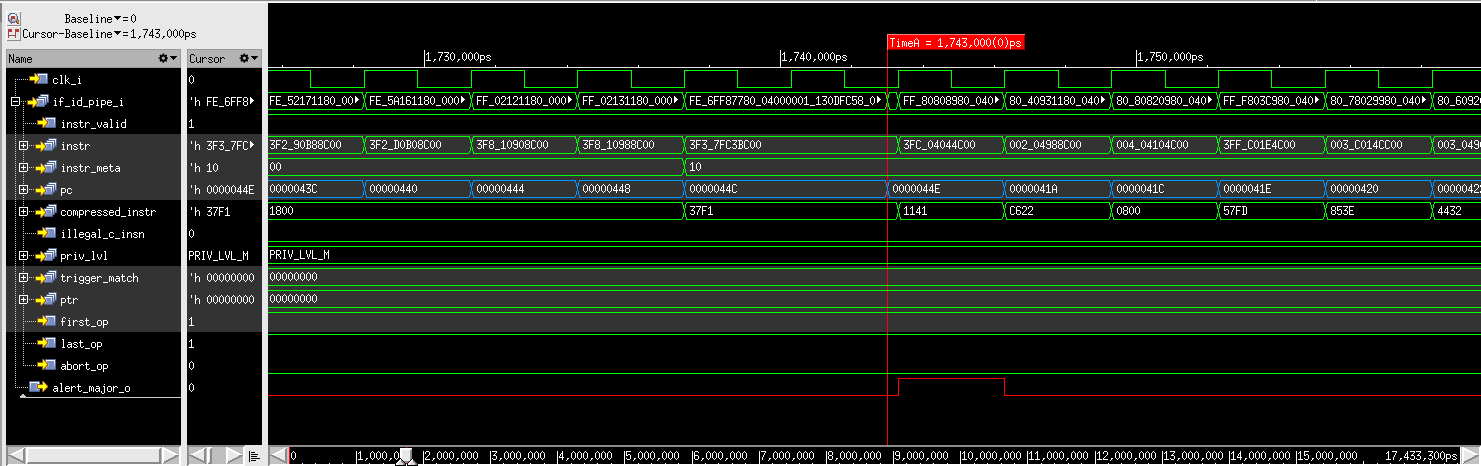
\includegraphics[width=\textwidth]{docs/images/instr_skip_glitch_injection_single_core.png}
    \caption{Waveforms from simulated skip of \textit{c.jal} instruction on CV32E40S.}
    \label{fig:instr_skip_single_wave}
\end{figure}

\subsubsection{Skipping out of while loop}

The \textit{c.j} instruction is logged in the \textit{WB} stage at 1833ns. The fault is injected in the \textit{EX} stage at 1824ns. The program counter is glitched to be \textit{0x0000047c}, thus skipping one instruction.

Glitching out of the while loop was not successful. The attempted instruction skip is detected and a major alert is raised. This can be seen in the simulation waveforms in \autoref{fig:instr_skip_loop_single_wave}. 

\begin{figure}[h!]
    \centering
    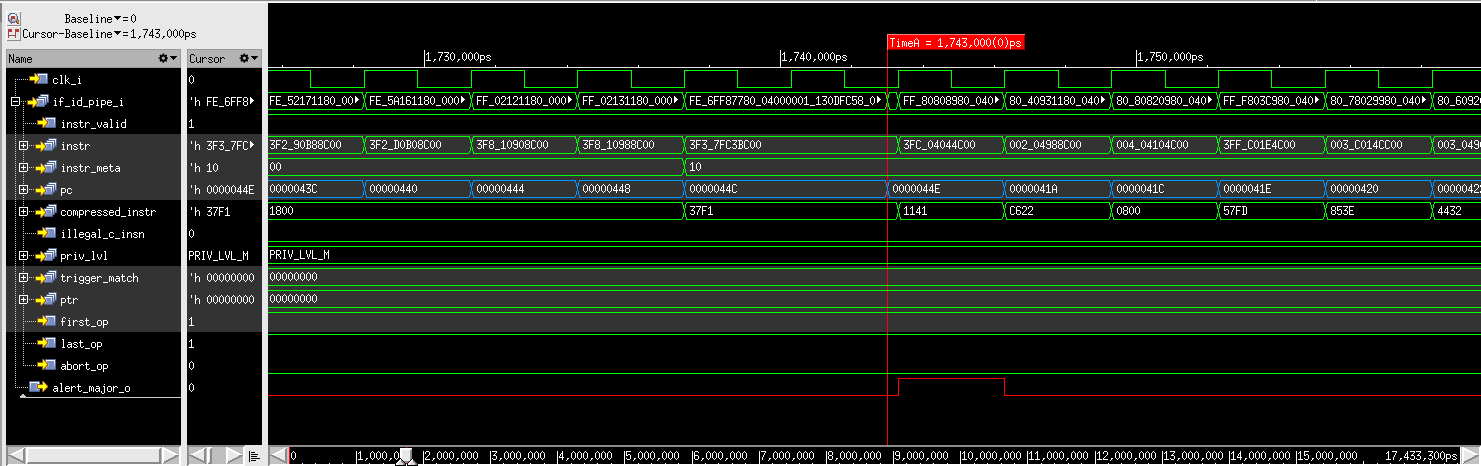
\includegraphics[width=\textwidth]{docs/images/instr_skip_glitch_injection_single_core.png}
    \caption{Waveforms from simulated skip of \textit{c.j} instruction to out of loop on CV32E40S.}
    \label{fig:instr_skip_loop_single_wave}
\end{figure}

\subsubsection{Skipping directly to end}

The call to the \textit{main} function is logged in the \textit{WB} stage at 1737ns. The fault is injected in the \textit{EX} stage at 1728ns. The program counter is glitched to the address \textit{0x00000482}, thus skipping 24 instructions.

This glitch attack was not successful. However, no major alert was raised by the core as can be seen in \autoref{fig:direct_skip_single_wave}. This glitch therefore bypassed the PCH feature. 

\begin{figure}[h!]
    \centering
    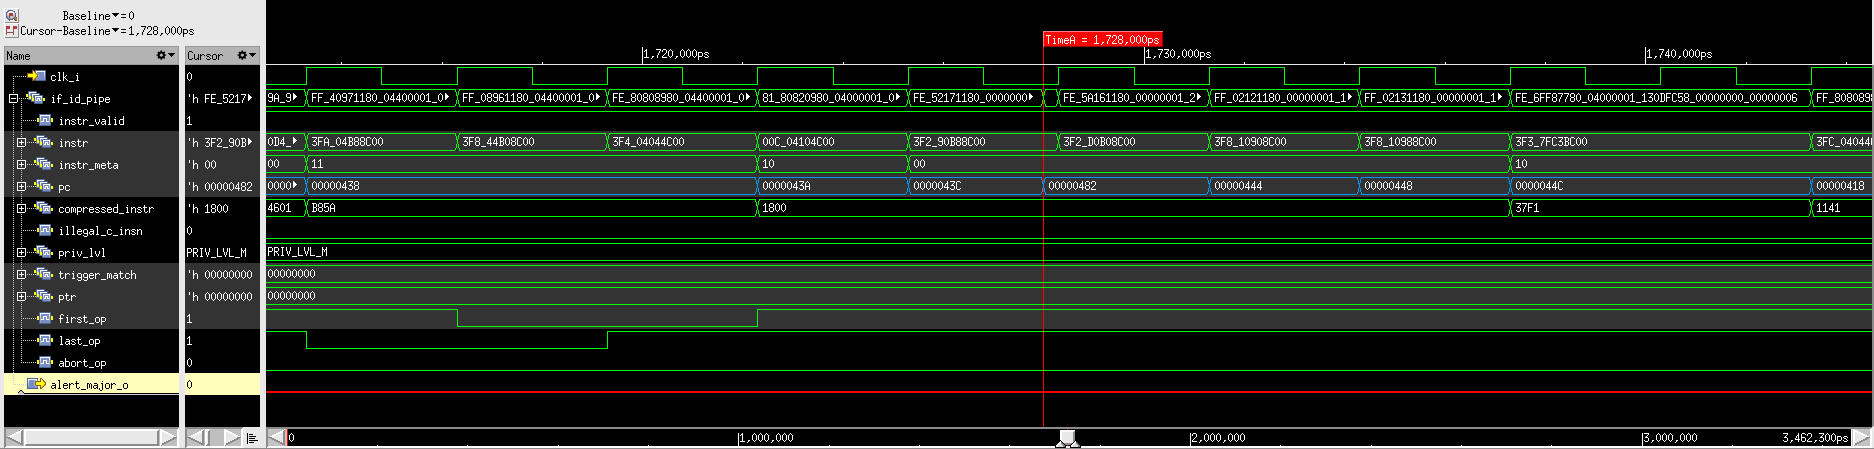
\includegraphics[width=\textwidth]{docs/images/direct_skip_single_core.png}
    \caption{Waveforms from simulated direct instruction skip on CV32E40S.}
    \label{fig:direct_skip_single_wave}
\end{figure}

\subsection{CV32E40DC}
\label{subsec:dual_instr_skip}

\subsubsection{Skipping function call}

The \textit{c.jal} instruction is logged in the \textit{WB} stage at 1707ns. The fault is injected in the \textit{EX} stage at 1698ns. The program counter is glitched to the address \textit{0x0000044e}, thus skipping one instruction. 

The glitch attack was not successful. From \autoref{fig:instr_skip_loop_dual_wave} we observe that the fault is detected immediately and the error propagates through each stage of the pipeline. 

\begin{figure}[h!]
    \centering
    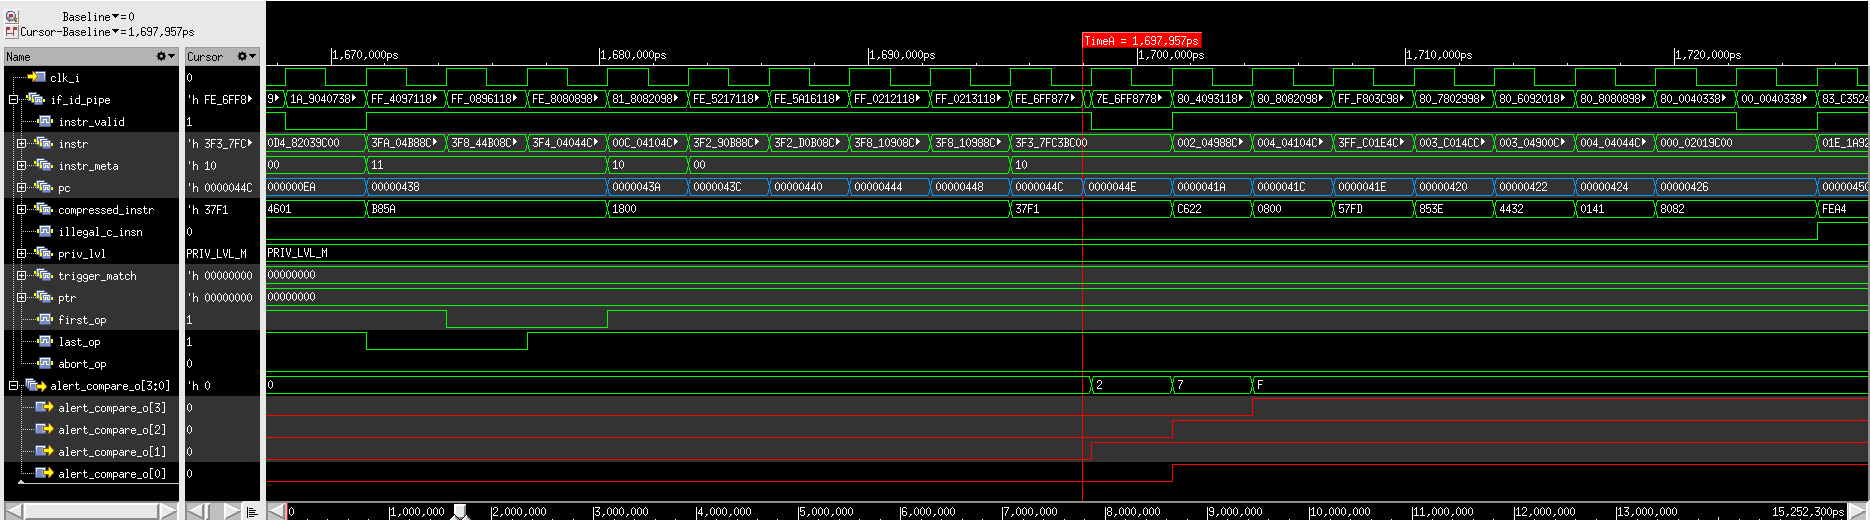
\includegraphics[width=\textwidth]{docs/images/instr_skip_dual_core.png}
    \caption{Waveforms from simulated skip of \textit{c.jal} instruction on CV32E40DC.}
    \label{fig:instr_skip_dual_wave}
\end{figure}


\subsubsection{Skipping out of while loop}

The \textit{c.j} instruction is logged in the \textit{WB} stage at 1782ns. The fault is injected in the \textit{EX} stage at 1773ns. The program counter is glitched to the address \textit{0x0000047c}, skipping one instruction.

The glitch attack was not successful. From \autoref{fig:instr_skip_loop_dual_wave} we observe that the fault is detected immediately and the error propagates though each stage of the pipeline. 

\begin{figure}[h!]
    \centering
    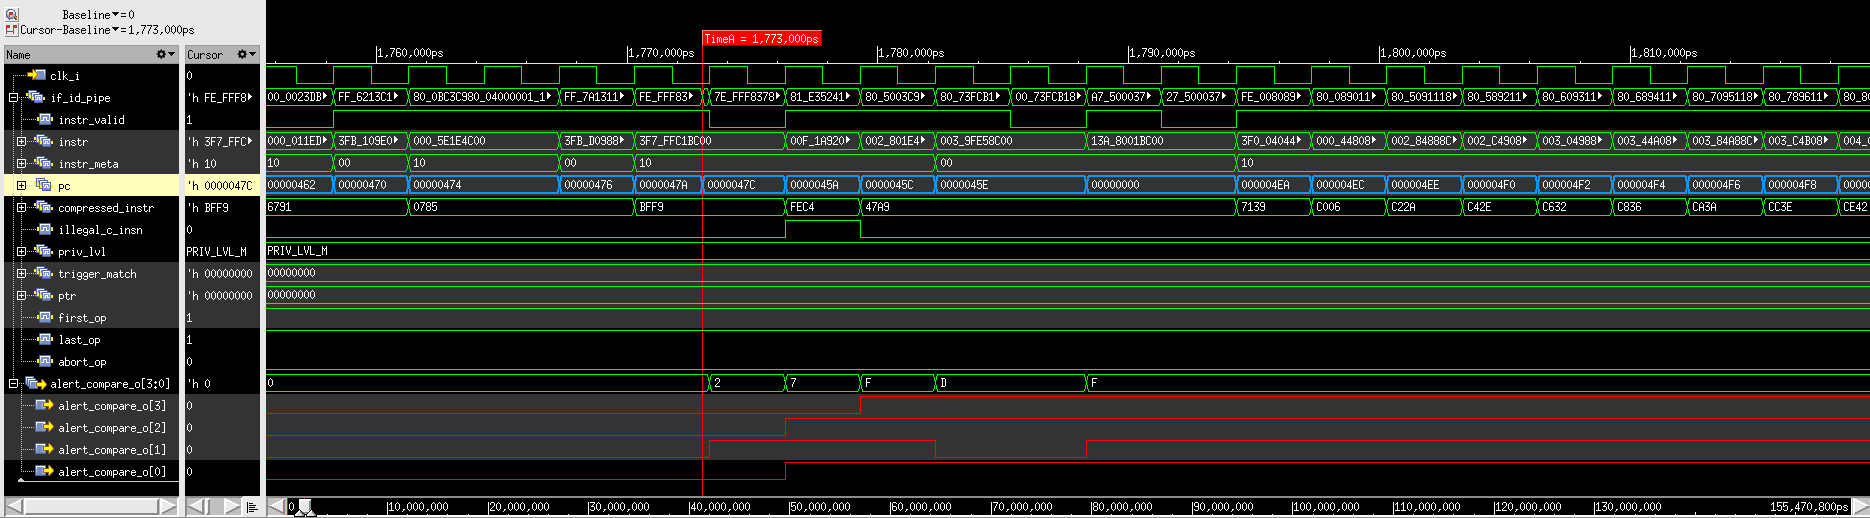
\includegraphics[width=\textwidth]{docs/images/instr_skip_loop_dual_core.png}
    \caption{Waveforms from simulated skip of \textit{c.j} instruction to jump out of loop on CV32E40DC.}
    \label{fig:instr_skip_loop_dual_wave}
\end{figure}

\subsubsection{Skipping directly to end}

The call to the \textit{main} function is logged in the \textit{WB} stage at 1689ns. The fault is injected in the \textit{EX} stage at 1680ns. The program counter is glitched to the address \textit{0x00000482}, thus skipping 24 instructions.

The glitch attack was not successful. From \autoref{fig:direct_skip_dual_wave} we observe that the fault is detected immediately and the error propagates through each stage of the pipeline. 

\begin{figure}[h!]
    \centering
    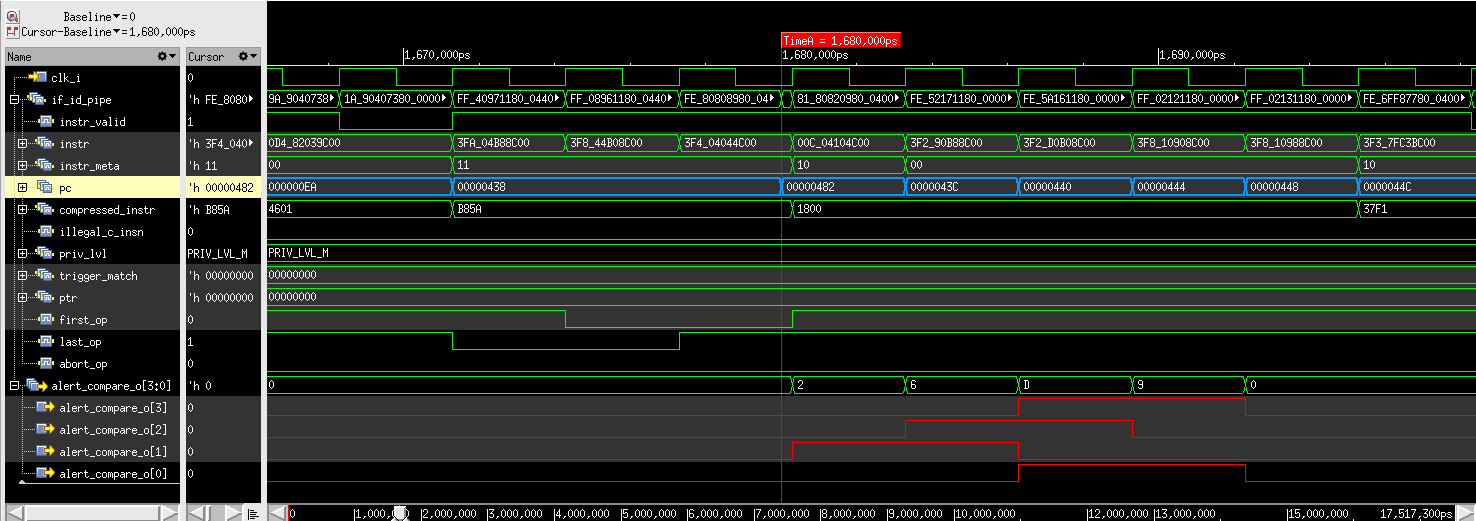
\includegraphics[width=\textwidth]{docs/images/direct_skip_dual_core.png}
    \caption{Waveforms from simulated direct instruction skip on CV32E40DC.}
    \label{fig:direct_skip_dual_wave}
\end{figure}


\section{Coverage Test}
\label{sec:cov_test_result}

\subsection{CV32E40S}

\subsubsection{Glitching load instruction}

The \textit{lw} instruction is logged in the \textit{WB} stage at 1827ns. The fault is also injected at 1827ns. The glitch attack was successful and the wrong value for the Fibonacci number was calculated. From \autoref{fig:lw_glitch_single_wave} we see that no major alert was raised by the single core, and the glitch goes undetected. 

\begin{figure}[h!]
    \centering
    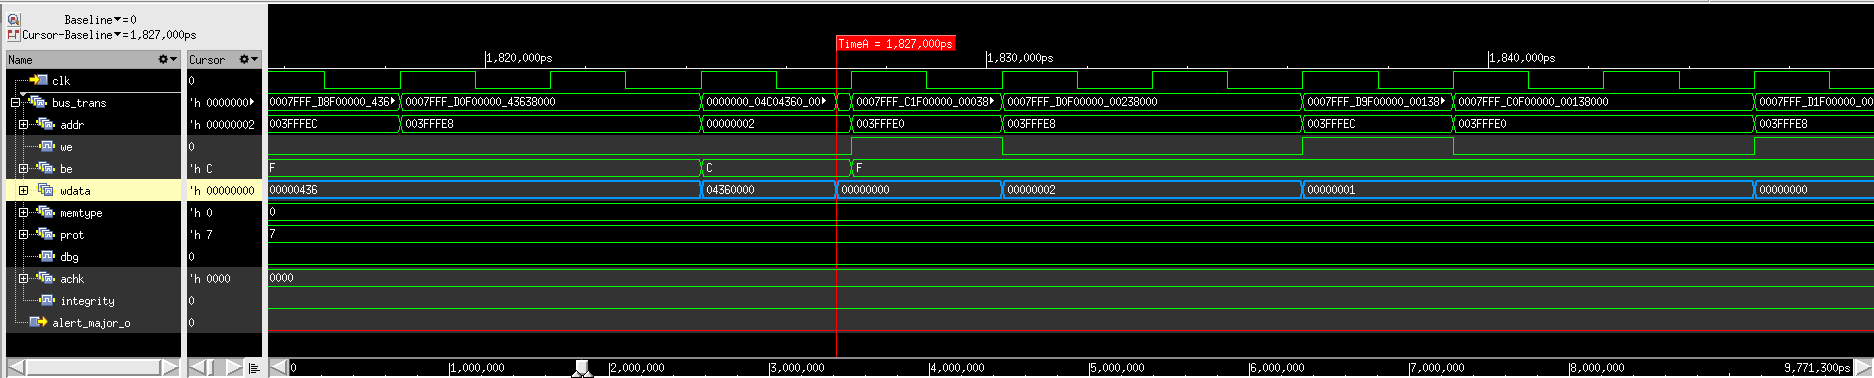
\includegraphics[width=\textwidth]{docs/images/lw_glitch_single_core.png}
    \caption{Waveforms from simulated glitched LW instruction skip on CV32E40S.}
    \label{fig:lw_glitch_single_wave}
\end{figure}

\subsubsection{Glitching store instruction}

The \textit{sw} instruction is logged in the \textit{WB} stage at 1836ns. The fault is also injected at 1836ns. The glitch attack was successful and the wrong value for the Fibonacci number was calculated. From \autoref{fig:sw_glitch_single_wave} we see that no major alert was raised by the single core, and the glitch goes undetected. 

\begin{figure}[h!]
    \centering
    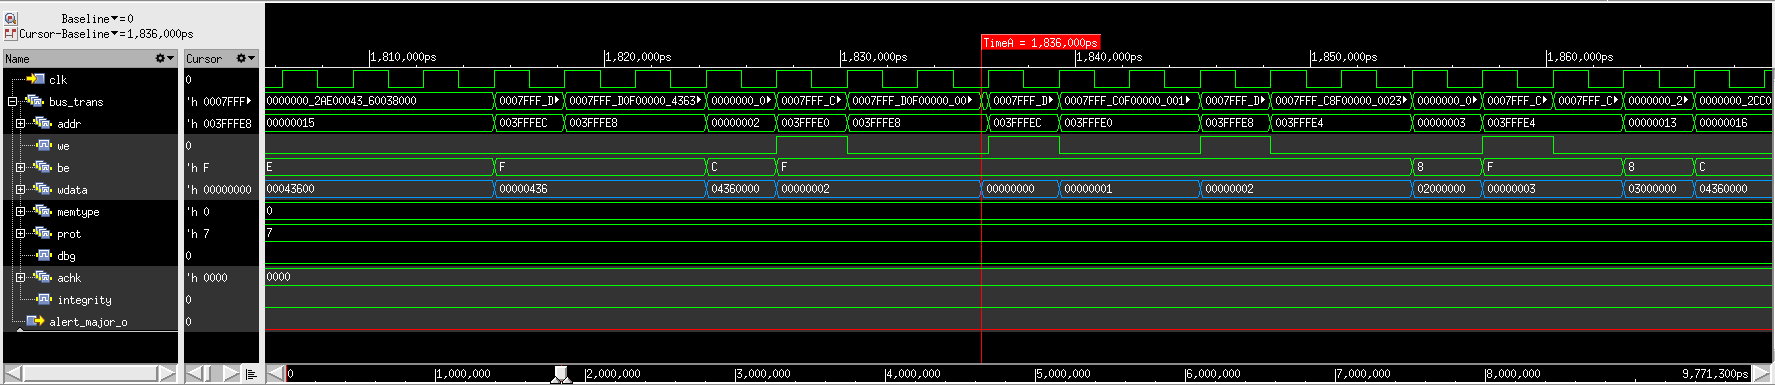
\includegraphics[width=\textwidth]{docs/images/sw_glitch_single_core.png}
    \caption{Waveforms from simulated glitched SW instruction skip on CV32E40S.}
    \label{fig:sw_glitch_single_wave}
\end{figure}


\subsection{Dual-Core Lockstep}

\subsubsection{Glitching load instruction}

The \textit{lw} instruction is logged in the \textit{WB} stage at 1722ns. The fault is also injected at 1722ns. The glitch attack was successful and the wrong value for the Fibonacci number was calculated. From \autoref{fig:lw_glitch_dual_wave} we see that bit \textit{0} on the \textit{alert\_compare\_o} bus is raised, meaning the system has detected a glitch in an OBI interface. 

\begin{figure}[h!]
    \centering
    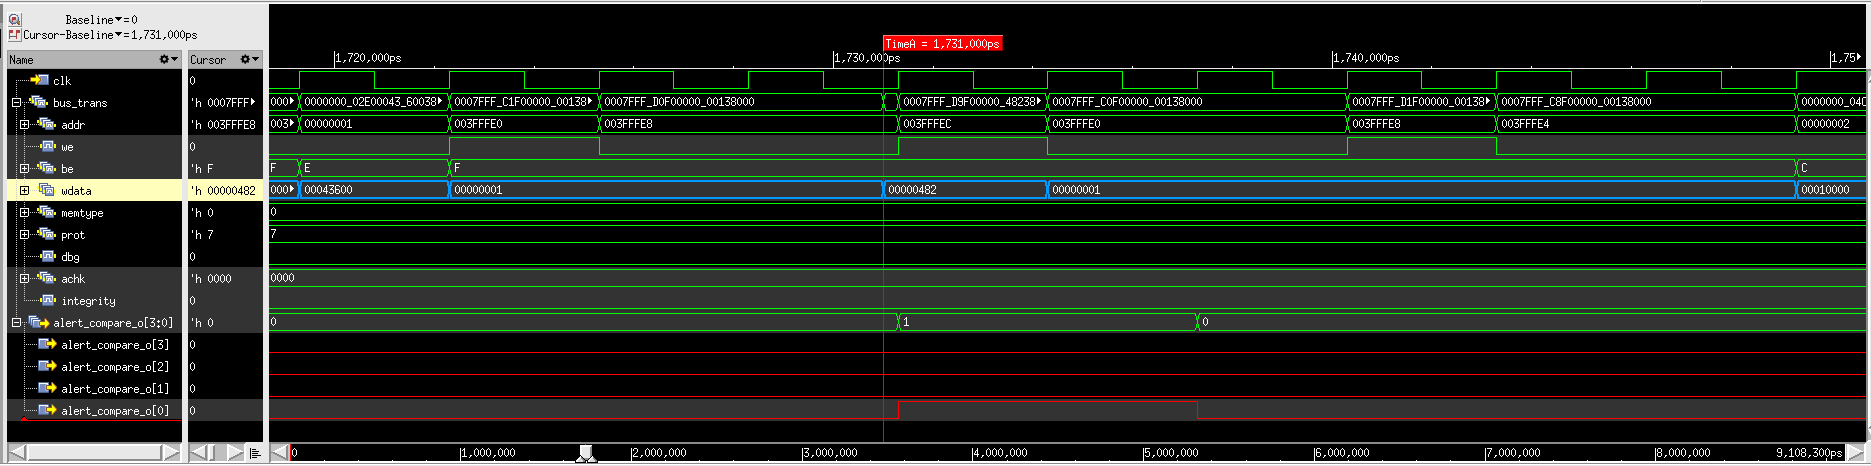
\includegraphics[width=\textwidth]{docs/images/lw_glitch_dual_core.png}
    \caption{Waveforms from simulated glitched LW instruction skip on Dual-Core Lockstep setup.}
    \label{fig:lw_glitch_dual_wave}
\end{figure}

\subsubsection{Glitching store instruction}

The \textit{sw} instruction is logged in the \textit{WB} stage at 1731ns. The fault is also injected at 1731ns. The glitch attack was successful and the wrong value for the Fibonacci number was calculated. From figure \autoref{fig:sw_glitch_dual_wave} we see that bit \textit{0} on the \textit{alert\_compare\_o} bus is raised, meaning the system has detected a glitch in an OBI interface. 

\begin{figure}[h!]
    \centering
    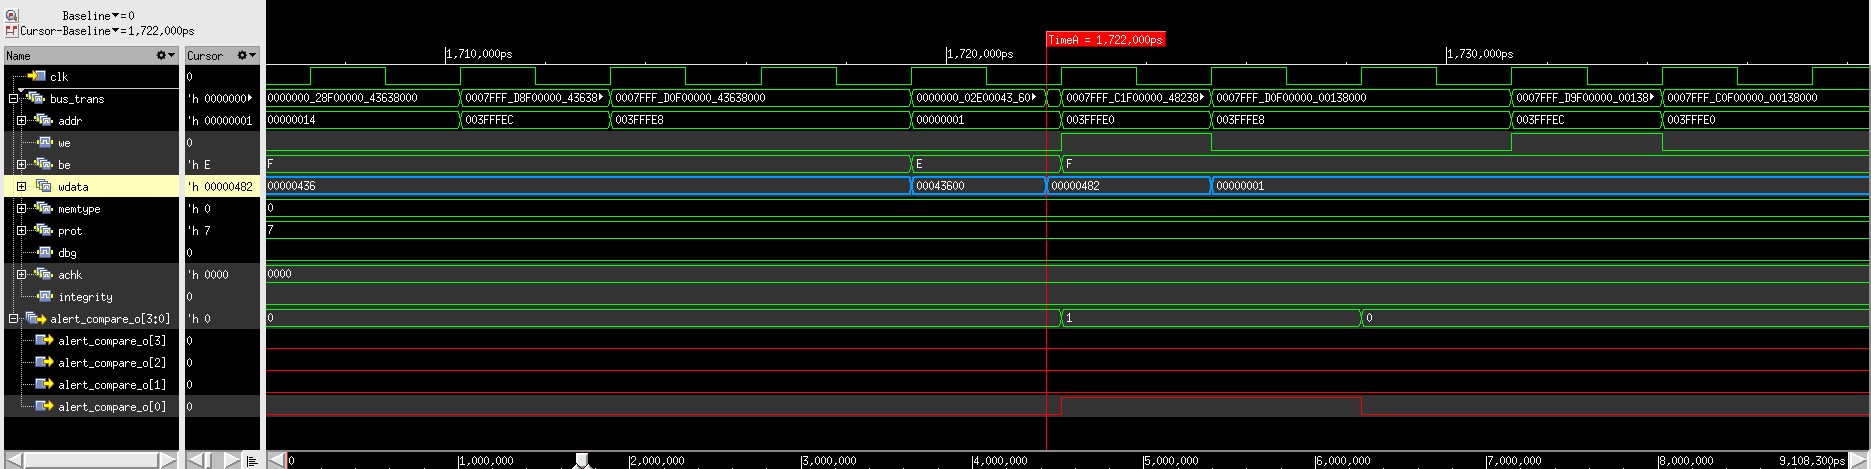
\includegraphics[width=\textwidth]{docs/images/sw_glitch_dual_core.png}
    \caption{Waveforms from simulated glitched SW instruction skip on Dual-Core Lockstep setup.}
    \label{fig:sw_glitch_dual_wave}
\end{figure}

\section{Discussion}
\label{sec:discussion}

As discussed in \autoref{sec:xsecure}, removing the PCH feature from the \textit{Xsecure} extension would lead to an increase in execution speed as shown in \autoref{tab:ppa_results} and \autoref{tab:test_ccs}. However, as mentioned previously this increase is limited by the side-channel attack prevention that also exists within the core. Exactly why the decrease in clock cycles from the CV32E40S to the CV32E40DC is always 9 is yet to be determined. This is not explained in the documentation for the core.  

Adding an extra core is also shown to add area and power consumption. \autoref{fig:area_power_plot} shows the difference between these metrics for both cores. The red bars represent the measured values from the CV32E40DC and the blue represent those from the CV32E40S. The axis on the left shows the area starting from 60000$pm^2$, and the axis on the right shows the power consumption in $\mu W$. The increase in area is smaller than the increase in power usage relative to the CV3E40S. The reason for this is that the CV32E40DC mainly adds computationally heavy logic circuits. These circuits will not necessarily occupy a lot area, but as shown in \autoref{sec:synth_comparison}, the dynamic power consumption from switching increases from $54.75\%$ to $63.42\%$. With optimization of the CV32E40DC, it is possible to bring these metrics closer to those of the CV32E40S. Doing this will save costs when producing and running the core and make it a more viable alternative to the CV32E40S. 

\begin{figure}[h!]
    \centering
    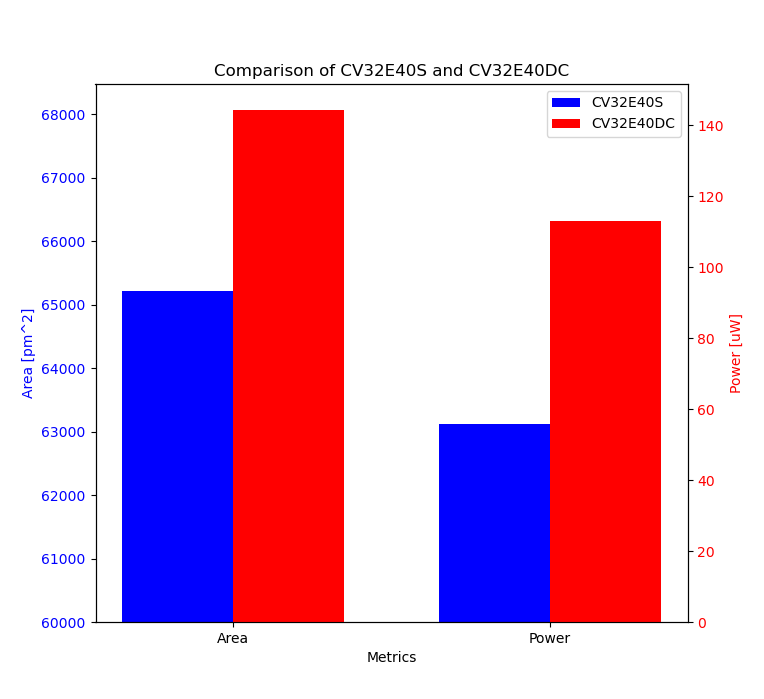
\includegraphics[width=0.55\textwidth]{docs/images/area_power_both_cores.png}
    \caption{Area and power consumption of synthesized CV32E40S and CV32E40DC cores. }
    \label{fig:area_power_plot}
\end{figure}

\autoref{tab:detection} shows the whether the glitch attack was detected or not for all tests. Detecting instruction skips is shown to be more reliable using the CV32E40DC. This core was able to detect a glitch in all three test cases. The CV32E40S was only able to detect a glitch in two of the three tests, as the glitch skipping directly to the end went undetected. For unknown reasons, the skipping of a function call was only successful on the CV32E40S as shown in \autoref{subsubsec:func_call}. Repeating the test lead to the same result every time. Random chance can therefore be ruled out. The reason why this test has a different outcome on both cores could be due to some undiscovered difference in timing between them.


\begin{table}[h]
\centering
\caption{Result of glitch detection in the tests from \autoref{tab:coverage_test} and \autoref{tab:instr_skip_test} on the CV32E40S and CV32E40DC.}
\label{tab:detection}
\setlength{\tabcolsep}{10pt} % Default value: 6pt
\renewcommand{\arraystretch}{1.5} % Default value: 1
\begin{tabular}{c|ccc}
\toprule 
Test                                                & CV32E40S                                      & CV32E40DC             \\     
\midrule 
\rowcolor{black!20} {Skipping function call}        & {\cellcolor[HTML]{34FF34}}{Detected} & {\cellcolor[HTML]{34FF34}}{Detected} \\ 
                    {Skipping out of while loop}    & {\cellcolor[HTML]{34FF34}}{Detected} & {\cellcolor[HTML]{34FF34}}{Detected} \\
\rowcolor{black!20} {Skipping directly to end}      & {\cellcolor[HTML]{CB0000}}{Not detected} & {\cellcolor[HTML]{34FF34}}{Detected} \\ 
                    {Glitching load instruction}    & {\cellcolor[HTML]{CB0000}}{Not detected} & {\cellcolor[HTML]{34FF34}}{Detected} \\ 
\rowcolor{black!20} {Glitching store instruction}   & {\cellcolor[HTML]{CB0000}}{Not detected} & {\cellcolor[HTML]{34FF34}}{Detected} \\
\bottomrule
\end{tabular}
\end{table}

For the coverage test it is clear that the CV32E40DC outperforms the CV32E40S as it is able to detect both glitch attacks. The CV32E40S detects neither of them. This is to be expected as these tests specifically target areas that are not covered by \textit{Xsecure}. This added coverage means that previously successful glitch attacks like those described in \autoref{chap3} might now be stopped. For example, the MTVEC exploit\cite{mtvec_corruption} would now be much more complex to perform. First of all an attacker would now need to trigger an exception in both cores. The timing offset between them makes this task more complicated. In addition the exception will need to be identical between the two cores, as any discrepancy will be detected. 